\documentclass[tikz]{standalone}
\usetikzlibrary{shapes,arrows.meta}
\begin{document}
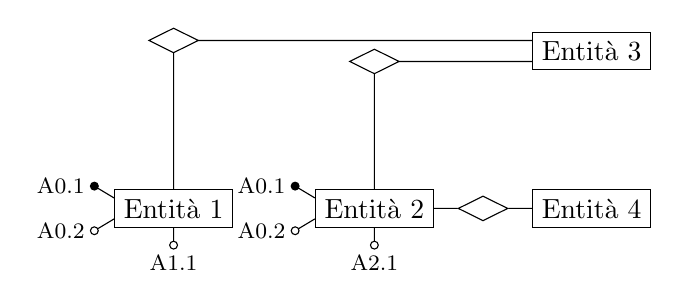
\begin{tikzpicture}
    \draw

    %%* Attributi:
    %%  node[draw, circle, inner sep=1pt,anchor=180, fill=black]{}node[right]{\footnotesize A}
    %%? Distanza orizzontale: E -(0.25,0.x)- A
    %%? Distanza verticale: E -(0,x * 0.22)- A

    %%* Cardinalità:
    %%  node[below right]{\scriptsize $(0,N)$}
    %%  node[above right]{\scriptsize $(0,N)$}
    %%  node[midway, above]{\scriptsize $(0,N)$}

    %%* Relazione:
    %%  node[draw, diamond, shape aspect=2, inner sep=3pt, anchor=90](r1){}
    %%  node[draw, diamond, shape aspect=2, inner sep=0.2pt, anchor=180](r2){R2}

    %%* Entità:
    %%  node[draw, rectangle, anchor=90](e1){}
    %%? Distanza verticale: E -(0.3)- R -(0.3) E
    %%? Distanza orizzontale: E -(0.75)- R -(0.75)- E


    (0,-1)++(-1.25,0)node[draw, rectangle, anchor=90](e1){Entità 1}
    (e1.170)--++(-0.25,.15)node[draw, circle, inner sep=1pt, fill=black]{}node[left]{\footnotesize A0.1}
    (e1.190)--++(-.25,-.15)node[draw, circle, inner sep=1pt, fill=white]{}node[left]{\footnotesize A0.2}

    (0,-1)++(1.3,0)node[draw, rectangle, anchor=90](e2){Entità 2}
    (e2.170)--++(-0.25,.15)node[draw, circle, inner sep=1pt, fill=black]{}node[left]{\footnotesize A0.1}
    (e2.190)--++(-.25,-.15)node[draw, circle, inner sep=1pt, fill=white]{}node[left]{\footnotesize A0.2}

    (e1.270)--++(0,-0.22)node[draw, circle, inner sep=1pt, fill=white]{}node[below]{\footnotesize A1.1}
    (e2.270)--++(0,-0.22)node[draw, circle, inner sep=1pt, fill=white]{}node[below]{\footnotesize A2.1}

    (e2.0)--++(0.3,0)node[draw, diamond, shape aspect=2, inner sep=3pt, anchor=180](r2){}
    (r2.0)--++(0.3,0)node[draw, rectangle, anchor=180](e4){Entità 4}

    (e4.90)++(0,2)node[draw, rectangle, anchor=90](e3){Entità 3}

    (e1.90)|-(e3.170)node[draw, fill=white, midway, diamond, shape aspect=2, inner sep=3pt](r3){}    
    (e2.90)|-(e3.190)node[draw, fill=white, midway, diamond, shape aspect=2, inner sep=3pt](r3){}
    ;
\end{tikzpicture}
\end{document}